%
% Sección de TES, capítulo de análisis y diseño de generación de tokens
% Proyecto Lovelace.
%

\section{\textit{Tweakable Encyphering Eschemes} (TES)}
\label{sec:tes}

La información que aquí se presenta puede ser consultada con mayor detalle en
\cite{cifradores_de_disco} y \cite{tweaks}.

La principal motivación para el diseño de \gls{gl:tes} son los \gls{gl:tbc},
los cuales fueron pensados como un medio de proveer de variabilidad a
los cifrados por bloques. En el esquema original, un cifrado por bloques es
totalmente determinístico: para el mismo mensaje y la misma llave, el texto
cifrado generado es siempre el mismo. Los \gls{gl:tbc} agregan un
\textit{tweak} a la entrada de un cifrador por bloques para darle
variabilidad; de esta manera, una misma llave y un mismo mensaje, ya no
producen siempre el mismo texto cifrado. El papel del \textit{tweak} es
bastante similar al del \gls{gl:vector_de_inicializacion}, solo que este
último opera a nivel de los modos de operación.

Es importante resaltar las diferencias entre el papel del \textit{tweak} y el
papel de la llave: esta provee de incertidumbre a un adversario,
mientras que el \textit{tweak} proporciona variabilidad. Mantener el
\textit{tweak} en secreto no debería proporcionar mayores niveles de
seguridad; de hecho, una condición en el diseño de \gls{gl:tbc} es que la
seguridad del cifrado por bloques no se ve incrementada (ni decrementada) por
la introducción del \textit{tweak}.

En la ecuación \ref{eq:tbc} se muestra la firma para un cifrado por bloques
con un \textit{tweak}. Comparando esta función con la de la ecuación
\ref{cifrado_bloques_def} (véase sección de cifrados por bloques,
\ref{sec:bloques}) se agrega un conjunto más al producto cruz de la entrada:
una cadena de bits de tamaño $ t $ (el espacio de los \textit{tweaks}).
\begin{equation}
  \label{eq:tbc}
  \tilde{E}: \{0,1\}^k \times \{0,1\}^y \times \{0,1\}^n
  \longrightarrow \{0,1\}^n
\end{equation}

En las siguientes ecuaciones se muestran algunas de las construcciones para
\gls{gl:tbc} propuestas a la fecha:
\begin{align}
  \label{tbc_trivial}
  \tilde{E}_k(T, M) &= E_k(T \oplus E_k(M)) \\
  \label{tbc_lrw}
  \tilde{E}_{k, h}(T, M) &= E_k(M \oplus h(T)) \oplus h(T) \\
  \label{tbc_we}
  \tilde{E}_{k}(T, M) &= E_k(M \oplus E_k(T)) \\
  \label{tbc_xex}
  \tilde{E}_{k}(T, M) &= E_k(M \oplus E_k(T)) \oplus E_k(T)
\end{align}

% TODO: ¿Qué es h()?
% Hmmm... ya sé que es (cuando menos sé cómo se define); sin embargo es
% más que nada cuestión matemática; creo que si se pone, obscurece
% inecesariamente el texto.
% h \in H
% En donde H es una familia de funciones e-AXU (allmost xor universal).
% Para que una función sea e-AXU se debe de cumplir que la probabilidad
% de que h(k, x) xor h(k, y) = z sea menor a e (para una llave aleatoria k).

Con los \gls{gl:tbc} se pueden crear modos de operación análogos a los que se
usan con los cifrados por bloques estándares. En la figura \ref{figura:tbc}
el \gls{gl:tbc_modo}, que es análogo a \gls{gl:cbc} (sección \ref{sec:cbc}).

\begin{figure}
  \centering
  \begin{subfigure}{0.45\textwidth}
    \begin{center}
      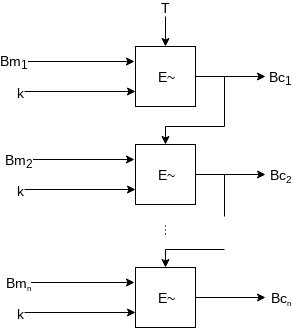
\includegraphics[width=0.7\linewidth]{diagramas/tbc.png}
      \caption{Cifrado.}
    \end{center}
  \end{subfigure}
  \begin{subfigure}{0.45\textwidth}
    \begin{center}
      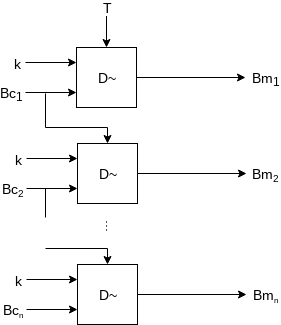
\includegraphics[width=0.7\linewidth]{diagramas/tbc_inverso.png}
      \caption{Descifrado.}
    \end{center}
  \end{subfigure}
  \caption{\Gls{gl:modo_de_operacion} \gls{gl:tbc_modo}.}
  \label{figura:tbc}
\end{figure}

Los \gls{gl:tbc} son usados para la construcción de \gls{gl:tes}. Para estos
existen dos clasificaciones: \textit{encrypt-mask-encrypt} y
\textit{hash-counter-hash}. En la primera clasificación se encuentran aquellos
que cuentan con dos capas de cifrado y una de enmascaramiento; algunos ejemplos
de esta son \gls{gl:cmc}, \gls{gl:eme} y \gls{gl:abl}. La segunda consiste en
dos funciones hash con un cifrado por bloques en modo de operación de contador
(sección \ref{sec:ctr}); algunos ejemplos son \gls{gl:xcb}, \gls{gl:hctr}
y HCH.

% ATENCIÓN, La pregunta de Sandra fué: ¿Cuál es la diferencia entre el
% tweak y un VI?
% Por si solos, son lo mismo: ambos son valores aleatorios públicos que
% introducen variabilidad. Me parece que la utilidad de los tweaks sobre los
% VI (y la de los modos de operación con tweaks sobre los tradicionales) va
% dada por las facilidades que introducen en el análisis y en el diseño
% de modos de operación. En honor a la verdad, aún no lo entiendo muy bien,
% pero eso es lo que dicen las conclusiones del artículo de Rivest.

La cuestión que queda por esclarecer ahora es, ¿cuál es la ventaja de utilizar
\gls{gl:tbc} en lugar de cifrados por bloques normales?, o en otro nivel,
¿cuál es la ventaja de utilizar \glspl{gl:modo_de_operacion} basados en
\textit{tweaks} a modos de operación con \glspl{gl:vector_de_inicializacion}?
Una primera impresión es que se trata de lo mismo: ambos, el \textit{tweak} y
el \gls{gl:vector_de_inicializacion}, son entradas extras que permiten
introducir variabilidad en los cifrados por bloques.

El primer punto clave es que los \textit{tweaks} introducen una división
semántica más en el análisis y diseño de modos de operación. En el esquema
tradicional solo existen dos divisiónes: el nivel bajo, referente a los
cifrados por bloques; y el nivel alto, referente a los modos de operación. Con
los \textit{tweaks}, el problema de los modos de operación se divide en dos:
cómo diseñar buenos \gls{gl:tbc}, y cómo diseñar buenos modos de operación
basados en \gls{gl:tbc}. Este nuevo enfoque permite filtrar nuevos problemas
en un nivel en particular sin que se afecten a las construcciones de los otros
niveles. El segundo punto clave es que los \gls{gl:tes} pueden ser diseñados
para recibir mensajesde longitud arbitraria y regresar cifrados de su misma
longitud.
